We use Linux Kernel version 3.5.0 for both application domain and driver
domains. We use the Arch Linux distribution for the \texttt{x86\_64}
platform for our testing and performance evaluation. The specifications of
the system used for the evaluation are presented in Table~\ref{tab:config}.

\begin{table}
\caption{Hardware specifications}
\begin{center}
\begin{tabular}{ll}
  \hline
  \label{tab:config}
  System Parameter & Configuration \\
  \hline
  Processor & 2 X Quad-core AMD Opteron(tm) Processor 2380, 2.49 Ghz \\
  Number of cores & 4 per processor \\
  Hyperthreading & OFF \\
  L1 L2 cache & 64K/512K per core \\
  L3 cache & 6144K \\
  Main memory & 16Gb \\
  Storage & SATA, HDD 7200RPM \\
  \hline 
\end{tabular}
\end{center}
\end{table}

\section{Goals}
\label{sec:goals}
The goals of our evaluation are:
\begin{enumerate}
\item \textbf{Comparison  of Xen's isolated driver domain mechanism with the interrupt-based IDDR system:}

In order to verify that the interrupt-based IDDR system constitutes a suitable baseline against 
which to compare the spinning-based IDDR system, we compared our interrupt-based implementation
against Xen's isolated driver domain.  However, since the source code
of the isolated driver domain implementation is not available, we achieve this evaluation goal 
by comparing the performance of the interrupt-based IDDR system with Xen's regular
drivers, which use the same split device driver model.

\item \textbf{Performance impact of spinning-based optimizations:}

The second goal of the evaluation is to prove that the spinning-based implementation of the 
communication channel improves the performance of the interdomain communication and hence the IDDR system.

We achieve this evaluation goal by comparing the performance of the interrupt-based IDDR system 
with the spinning-based IDDR system.
\end{enumerate}

\section{Methodology}
\label{sec:methodology}
In order to measure the performance of the system, we run performance
tests using a variety of block devices. In order to cover a variety of
devices we use block devices such as SATA disks, ramdisks and loop
devices for the performance testing. A loop device is a device that provides 
a block device that is backed by a file.  A ramdisk is a block of a memory
that acts as a disk drive.

In order to conduct the performance tests, we format the block
device with the ext2 file system, and run the SysBench
benchmark~\cite{sysbench} on it. SysBench is a multi-threaded benchmark
tool for evaluating operating system performance. It includes different test
modes, one of which is FileIO.  The FileIO mode can be used to produce
different file I/O workloads. It runs a specified number of threads to
execute requests in parallel. We run the SysBench benchmark in FileIO
test mode to generate 128 files with \texttt{1GB} of total data. We
execute random reads, random writes, and a mix of random reads and writes
on all three devices. We set the block size to \texttt{16KB}. We vary
the number of SysBench threads from 1 to 32 to measure the throughput of
the system under different levels of concurrent access.

\section{Xen Split Device Driver vs interrupt-based IDDR System}
As per our first evaluation goal discussed in Section~\ref{sec:goals},
we compare the interrupt-based IDDR system with Xen's split device driver.

\subsection*{Experimental Setup}

\subsubsection*{Xen Split Device Driver}
We create a ramdisk in domain 0. The guest domain (domain U) is configured
to access domain 0's ramdisk via a split device driver. 
We use the same setup for the loop device and the SATA disk. 
We format and mount the disk into a partition in the
guest domain using the ext2 file system in all cases. The SysBench 
benchmark is run on the mounted partitions as explained in 
Section~\ref{sec:methodology}.

\subsubsection*{Interrupt-based IDDR System}
In the Xen hypervisor, the domain 0 always runs as a paravirtualized guest (PV),
but domain U can be using both a hardware-assisted virtualization configuration (HVM) 
or a paravirtualized configuration.  In our setup we run domain U always
in HVM mode because HVM guests exhibit less system call overhead
and faster memory bandwidth compared to PV guests, as we observed
by running the system call micro-benchmark tool lmbench\cite{lmbench}. 

When comparing to Xen's split device drivers, the backend device driver executes
in domain 0 and the frontend device driver in domain U.  
To eliminate any performance differences that may be solely due the mode
of virtualization used, we matched the modes of virtualization
by running IDDR's backend and frontend drivers also in 
domain 0 and U, respectively.

\subsubsection*{Comparison}
We compare the throughput of Xen's split device driver and the
interrupt-based IDDR system in Figure~\ref{fig:iddrvsxen-ramdisk-rdwr}
and Figure~\ref{fig:iddrvsxen-loop-rd}. 
Figure~\ref{fig:iddrvsxen-ramdisk-rdwr} presents the
throughput of both systems when data is randomly read from a ramdisk and
written to it. Figure~\ref{fig:iddrvsxen-loop-rd} presents the throughput
when data is randomly read from a loop device.

On a loop device, the performance of the interrupt based IDDR system
differs by 3\%-4\% when compared to Xen's split device driver. On a
ramdisk, the throughput of the interrupt based IDDR system matches that
of the Xen split device driver. This shows that our interrupt-based
IDDR implementation provides a suitable baseline for our performance 
optimizations.

\begin{figure}[!ht]
%\centering
  \begin{subfigure}[b]{0.2\textwidth}
  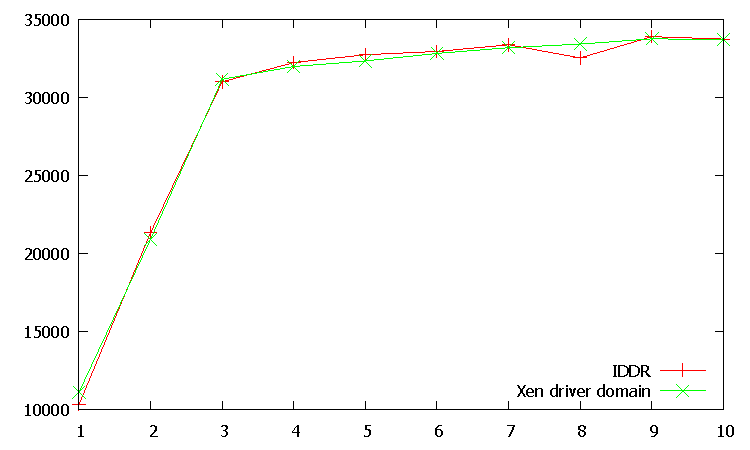
\includegraphics[scale=.7]{iddrvsxen-ramdisk-rdwr}
  \caption{Random reads-writes on a ramdisk}
  \label{fig:iddrvsxen-ramdisk-rdwr}
  \end{subfigure}
  \hspace{50mm}
  %\hfill
  \begin{subfigure}[b]{0.2\textwidth}
  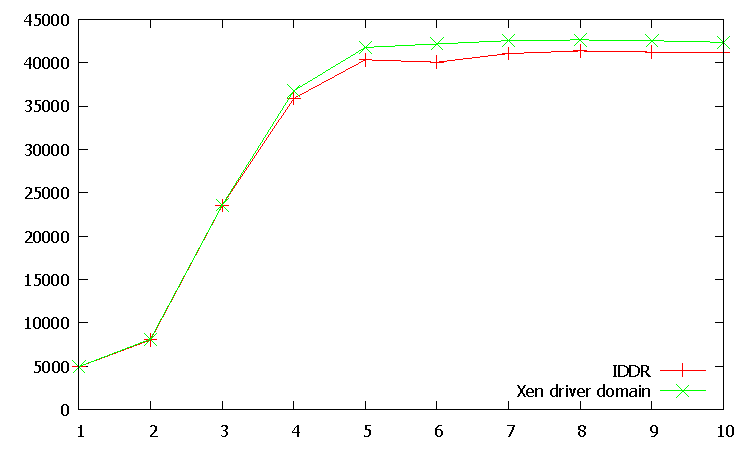
\includegraphics[scale=.7]{iddrvsxen-loop-rd}
  \caption{Random reads on a loop device}
  \label{fig:iddrvsxen-loop-rd}
  \end{subfigure}\\
\caption{Interrupt Based IDDR system vs Xen split driver}\label{fig:seqloopdisk}
\end{figure}

%
% CONTINUE HERE
%
\section{Interrupt Based IDDR System vs Spinning Based IDDR System}
We measure and compare the performance of the interrupt based IDDR system
with the spinning based IDDR system. To compare the performance of both
systems, we measure performance of the system by varying the number of
SysBench threads. The SysBench benchmark executes random read write on
a ramdisk and loop device.

\subsection*{Experimental Setup}
In both systems, the application domain is domain 0, and the driver domain
is domain U. We create a ramdisk and insert the backend driver in the
driver domain. We insert the frontend driver in the application domain.

We measure the performance of both systems on a loop device with same setup.

In order to use SATA disk in domain U we needed SATA controller of the
disk to passthrough. However because of technical issues we couldn't
passthrough SATA controller to domain U. Hence only for SATA disk
experiment we use domain 0 as a driver domain and domain U as an
application domain.

\subsubsection*{Random reads and writes}

\paragraph{Comparison :}

Figure~\ref{fig:rndramdisk}, Figure~\ref{fig:rndloopdisk} and Figure~\ref{fig:rndharddisk} compares the throughput of the interrupt based IDDR and the spinning based IDDR system when data is randomly read from a ramdisk, loop device, SATA disk and is written on them.

Figure~\ref{subfig:rndrd-ramdisk}, Figure~\ref{subfig:rndrd-loopdisk} Figure~\ref{subfig:rndrd-harddisk} show that the spinning based IDDR system performs better when data is read from a device randomly.  

Figure~\ref{subfig:rndwr-ramdisk}, Figure~\ref{subfig:rndwr-loopdisk} and Figure~\ref{subfig:rndwr-harddisk} compare the performance of the device when data is written randomly to a device. The graph shows that initially the spinning based IDDR system performs better than the interrupt based IDDR system, but as number of SysBench threads increases, the throughput of the spinning based IDDR system decreases.
\\[3mm] 
Figure~\ref{subfig:rndrw-ramdisk}, Figure~\ref{subfig:rndrw-loopdisk} and Figure~\ref{subfig:rndrw-harddisk} compare the performance for mix random read and write workload. 

\begin{figure}[!ht]
% \centering
  \begin{subfigure}[b]{0.2\textwidth}
  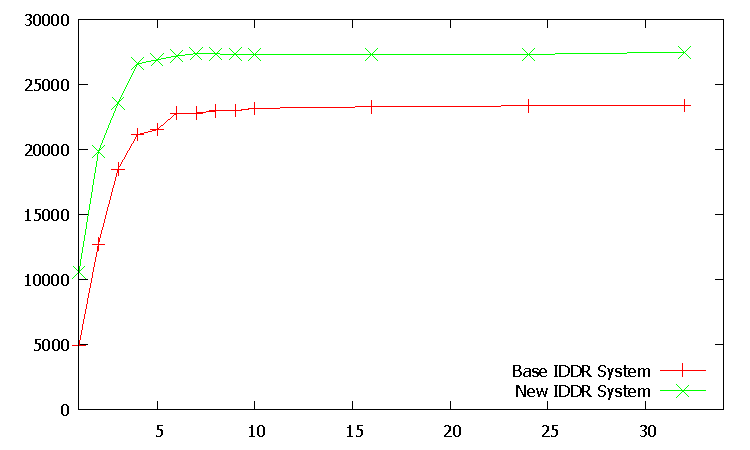
\includegraphics[scale=.7]{rndrd-ramdisk}
  \caption{Random reads}
  \label{subfig:rndrd-ramdisk}
  \end{subfigure}
  \hspace{50mm}
  \begin{subfigure}[b]{0.2\textwidth}
  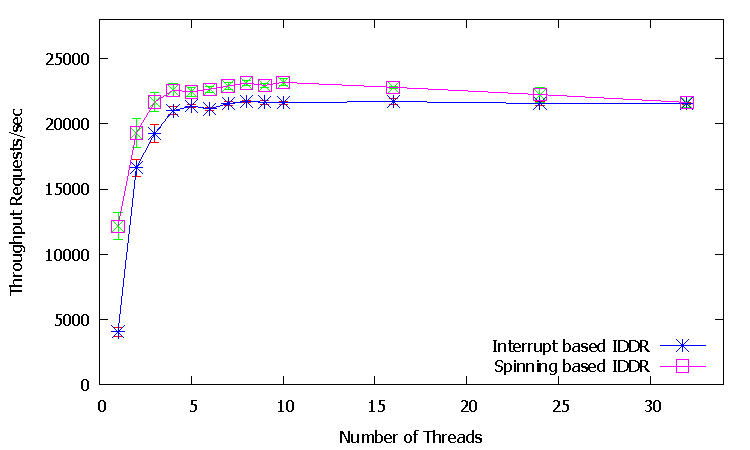
\includegraphics[scale=.7]{rndwr-ramdisk}
  \caption{Random writes}
  \label{subfig:rndwr-ramdisk}
  \end{subfigure}\\*
  \hspace{150mm}
  \begin{subfigure}[b]{0.3\textwidth}
  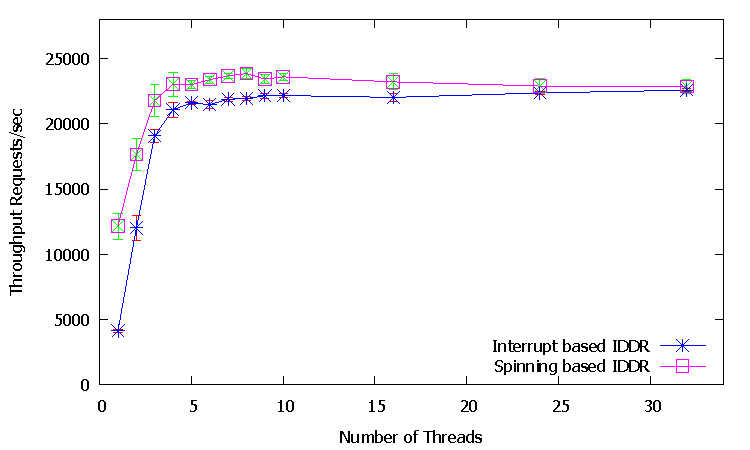
\includegraphics[scale=.7]{rndrw-ramdisk}
  \caption{Random reads writes}
  \label{subfig:rndrw-ramdisk}
  \end{subfigure}
  \caption{Random reads and writes on a Ramdisk}\label{fig:rndramdisk}
\end{figure}

\begin{figure}[!ht]
%\centering
  \begin{subfigure}[b]{0.2\textwidth}
  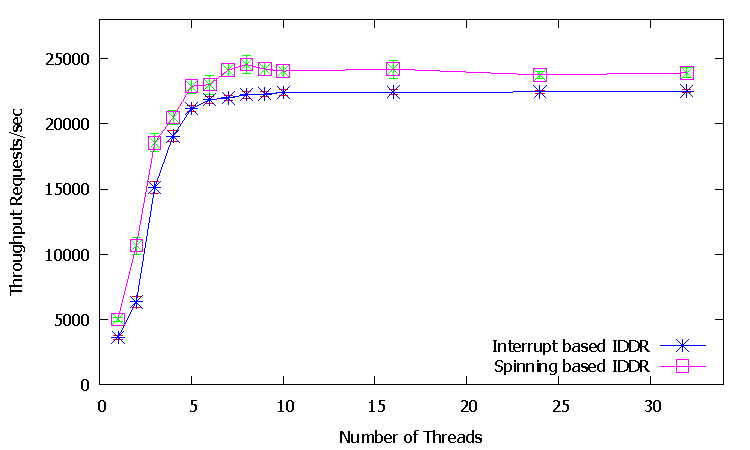
\includegraphics[scale=.7]{rndrd-loopdisk}
  \caption{Random reads}
  \label{subfig:rndrd-loopdisk}
  \end{subfigure}
  \hspace{50mm}
  \begin{subfigure}[b]{0.2\textwidth}
  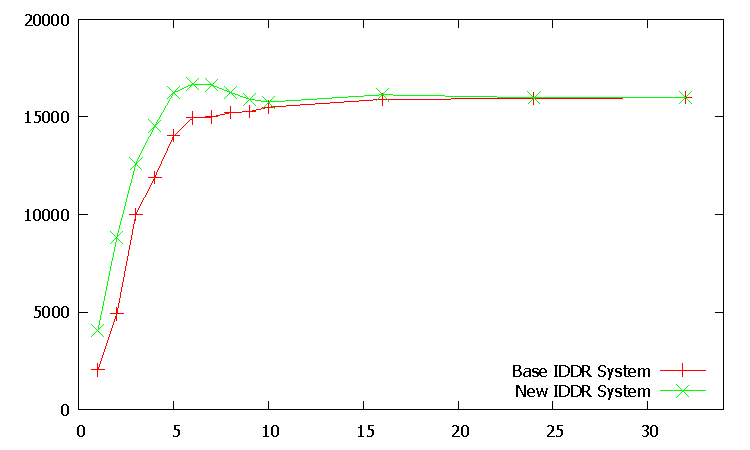
\includegraphics[scale=.7]{rndwr-loopdisk}
  \caption{Random writes}
  \label{subfig:rndwr-loopdisk}
  \end{subfigure}\\
  \begin{subfigure}[b]{0.3\textwidth}
  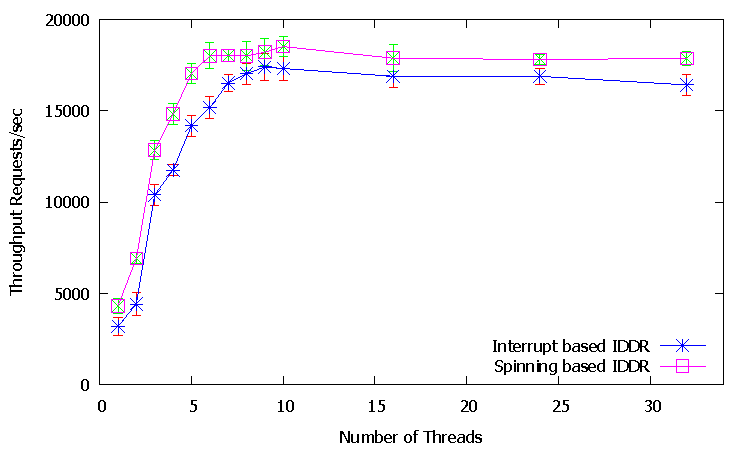
\includegraphics[scale=.7]{rndrw-loopdisk}
  \caption{Random reads writes}
  \label{subfig:rndrw-loopdisk}
  \end{subfigure}
\caption{Random reads and writes on a Loop device}\label{fig:rndloopdisk}
\end{figure}

\begin{figure}[!ht]
%\centering
  \begin{subfigure}[b]{0.2\textwidth}
  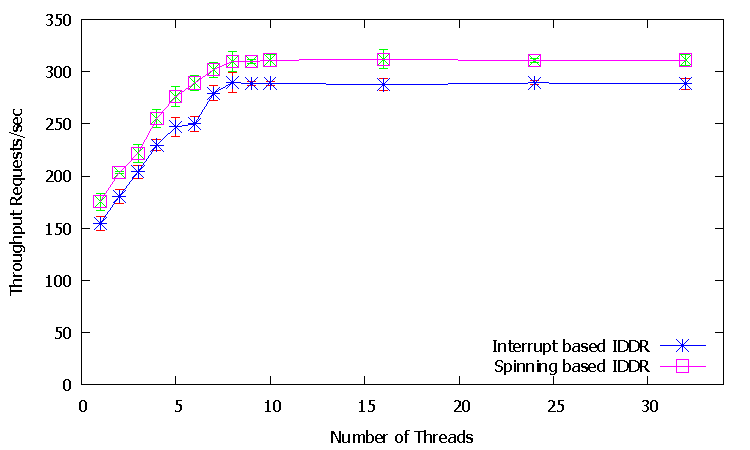
\includegraphics[scale=.7]{rndrd-harddisk}
  \caption{Random reads}
  \label{subfig:rndrd-harddisk}
  \end{subfigure}
  \hspace{50mm}
  \begin{subfigure}[b]{0.2\textwidth}
  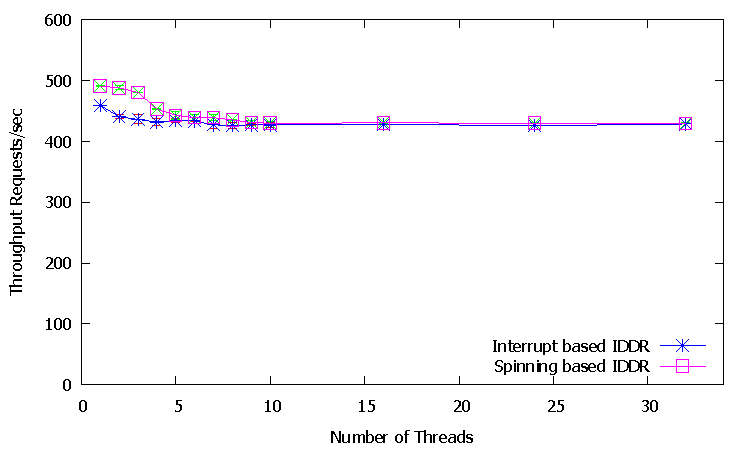
\includegraphics[scale=.7]{rndwr-harddisk}
  \caption{Random writes}
  \label{subfig:rndwr-harddisk}
  \end{subfigure}\\
  \begin{subfigure}[b]{0.3\textwidth}
  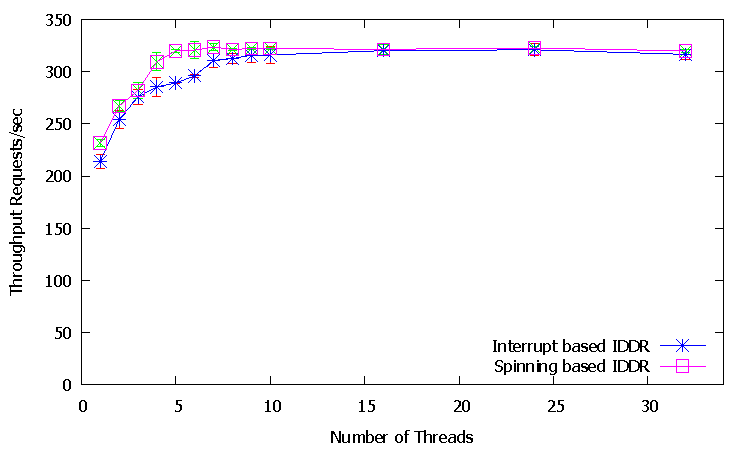
\includegraphics[scale=.7]{rndrw-harddisk}
  \caption{Random reads writes}
  \label{subfig:rndrw-harddisk}
  \end{subfigure}
\caption{Random reads and writes on a SATA disk}\label{fig:rndharddisk}
\end{figure}


\paragraph{Observation :}
The performance analysis of the interrupt based and spinning IDDR system shows that initially the throughput of the system increases and then it remains constant. We measure the throughput of the system with varying number of SysBench threads. 

In both the systems, when the number of SysBench threads is low, the rate at which data is read and written is low and when number of SysBench threads is high, the rate at which data is read and written is high. Low data workload results in low throughput and high data workload results in high data throughput. Once maximum throughput is achieved, it remains constant.

In interrupt based IDDR system, virtual interrupt is send between application domain and driver domain for read and write requests and in spinning based IDDR system, both the domains spin for the request and responses. Our optimization technique reduces the frequency of the virtual interrupt being sent between domains. Hence the improvement in performance depends upon number of virtual interrupts avoided. In the interrupt based IDDR system, when data workload is low, requests are generated with larger gaps of interval. Hence less number of requests are batched together, which results in more virtual interrupts. However, high workload observes more requests being batched together. Since spinning based IDDR system avoids more portion of virtual interrupts when workload is low, we observe a more performance gain when data workload is low. 

\subsubsection*{CPU utilization}

In spinning based IDDR system the frontend and backend driver spin for the request and responses and uses the CPU cycles. Hence we see a trade-off between high CPU utilization and high throughput. 

In this section we compare the CPU utilization of interrupt based and spinning based IDDR system.

Figure~\ref{fig:cpuramdisk}, Figure~\ref{fig:cpuloopdisk} and Figure~\ref{fig:cpuharddisk} compares the CPU performance of both the systems with ramdisk, loop device and SATA disk as a physical device. 

\paragraph{Observation: }
Since in IDDR system, read response thread and read request thread spin continuously both threads consume 2 cores of the system all the time. In below graphical presentation, 100\% CPU utilization denotes full utilization of 1 CPU. It can be seen that CPU utilization of spinning based system is near 200\% i.e. 2 cores. 

\begin{figure}[!ht]
%\centering
  \begin{subfigure}[b]{0.2\textwidth}
  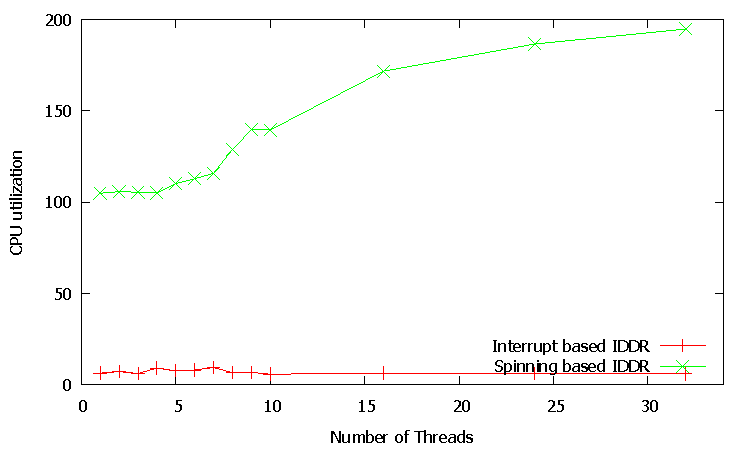
\includegraphics[scale=.7]{cpu-rndrd-ramdisk}
  \caption{Random reads}
  \label{subfig:cpu-rndrd-ramdisk}
  \end{subfigure}
  \hspace{50mm}
  \begin{subfigure}[b]{0.2\textwidth}
  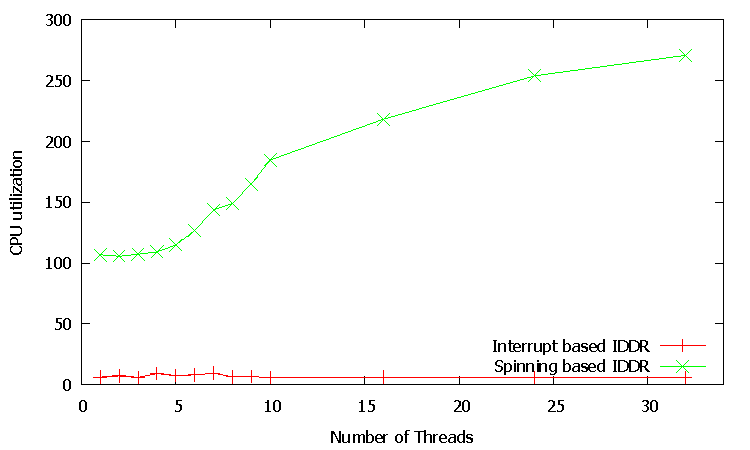
\includegraphics[scale=.7]{cpu-rndrw-ramdisk}
  \caption{Random writes}
  \label{subfig:cpu-rndrw-ramdisk}
  \end{subfigure}\\
  \begin{subfigure}[b]{0.3\textwidth}
  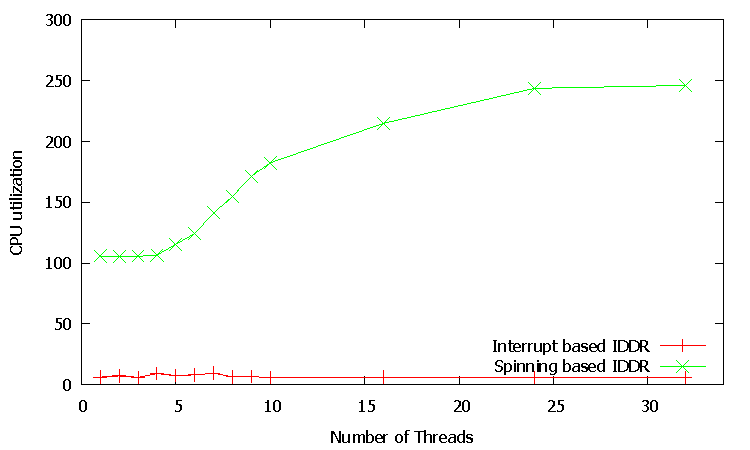
\includegraphics[scale=.7]{cpu-rndwr-ramdisk}
  \caption{Random reads writes}
  \label{subfig:cpu-rndwr-ramdisk}
  \end{subfigure}
\caption{Comparison of CPU utilization - ram disk}\label{fig:cpuramdisk}
\end{figure}

\begin{figure}[!ht]
  \begin{subfigure}[b]{0.2\textwidth}
  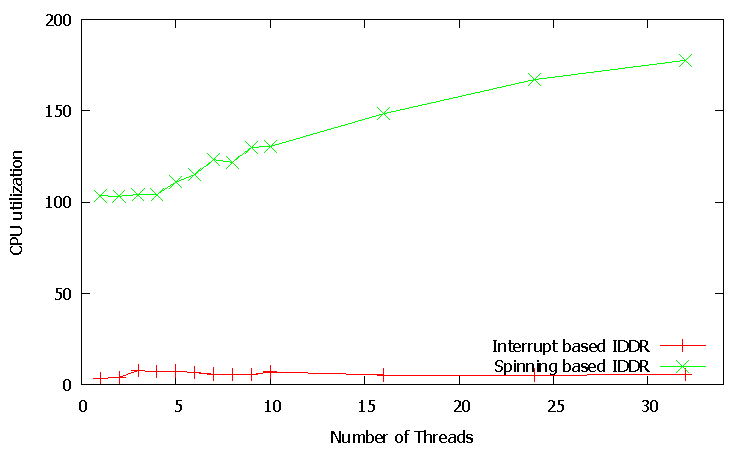
\includegraphics[scale=.7]{cpu-rndrd-loopdisk}
  \caption{Random reads}
  \label{subfig:cpu-rndrd-loopdisk}
  \end{subfigure}
  \hspace{50mm}
  \begin{subfigure}[b]{0.2\textwidth}
  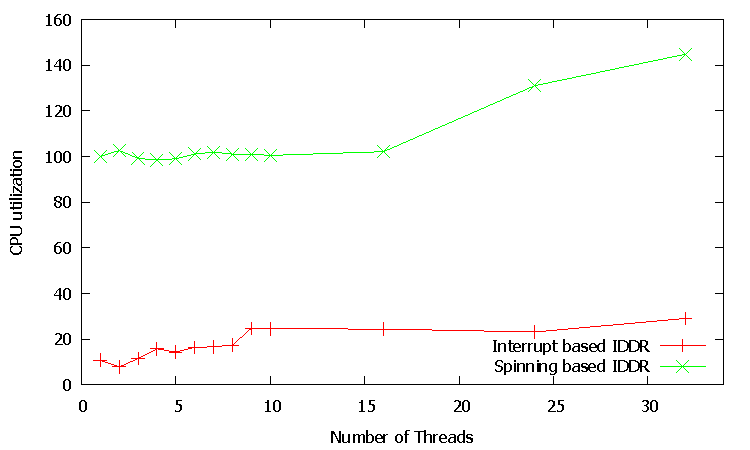
\includegraphics[scale=.7]{cpu-rndrw-loopdisk}
  \caption{Random writes}
  \label{subfig:cpu-rndrw-loopdisk}
  \end{subfigure}\\
  \begin{subfigure}[b]{0.3\textwidth}
  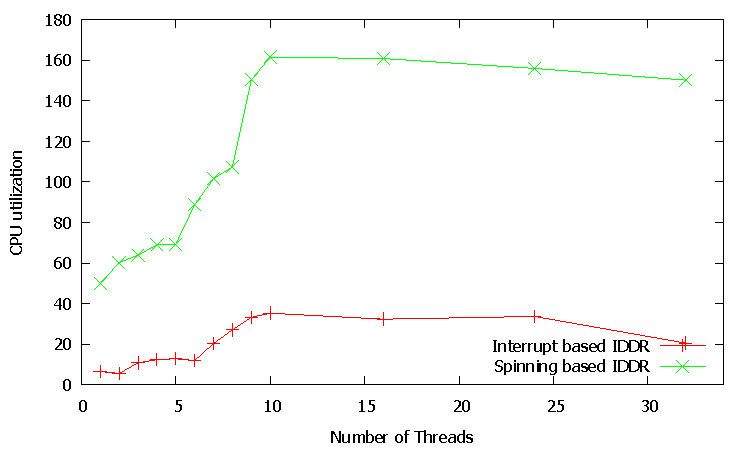
\includegraphics[scale=.7]{cpu-rndwr-loopdisk}
  \caption{Random reads writes}
  \label{subfig:cpu-rndwr-loopdisk}
  \end{subfigure}
\caption{Comparison of CPU utilization - loop device}\label{fig:cpuloopdisk}
\end{figure}

\begin{figure}[!ht]
%\centering
  \begin{subfigure}[b]{0.2\textwidth}
  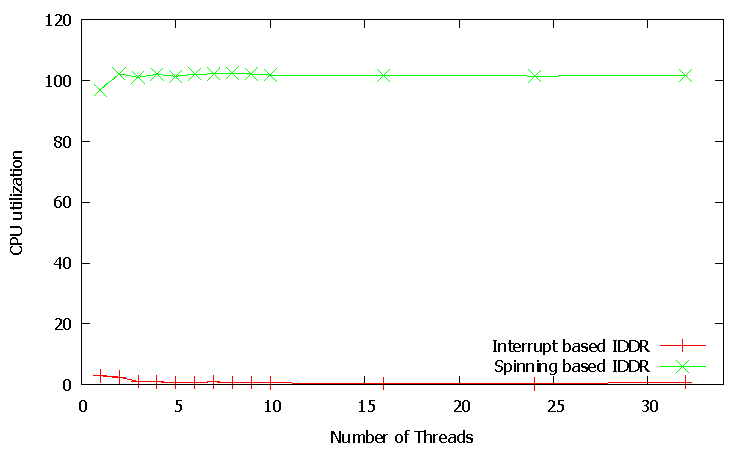
\includegraphics[scale=.7]{cpu-rndrd-harddisk}
  \caption{Random reads}
  \label{subfig:rndrd-harddisk}
  \end{subfigure}
  \hspace{50mm}
  \begin{subfigure}[b]{0.2\textwidth}
  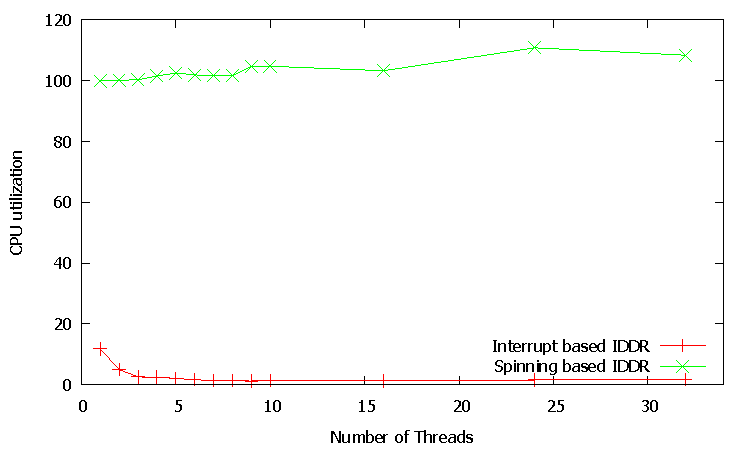
\includegraphics[scale=.7]{cpu-rndwr-harddisk}
  \caption{Random writes}
  \label{subfig:rndwr-harddisk}
  \end{subfigure}\\
  \begin{subfigure}[b]{0.3\textwidth}
  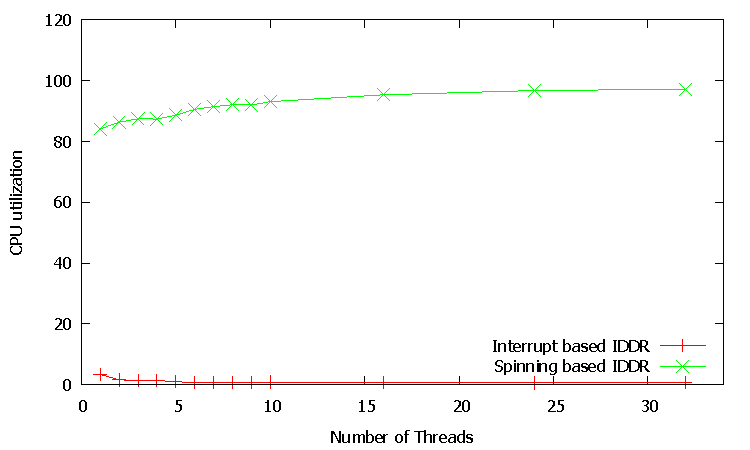
\includegraphics[scale=.7]{cpu-rndrw-harddisk}
  \caption{Random reads writes}
  \label{subfig:rndrw-harddisk}
  \end{subfigure}
\caption{Comparison of CPU utilization - SATA disk}\label{fig:cpuharddisk}
\end{figure}

